\documentclass[../main.tex]{subfiles}

\begin{document}
	
The View and Majority Vote based 3D scene retrieval algorithm (VMV) utilizes the VGG-16 architecture, as is illustrated in \textbf{Fig.}~\ref{SHREC19}. 

\subsubsection{3D Scene View Sampling}
Each 3D scene model is in a 3D sphere observable by an automated QMacro that captures 13 scene views. Of these 13 unique perspectives, 12 are uniformly sample along the equator of the sphere while the last view is from a top-down perspective as shown in \textbf{Fig.}~\ref{apartment_building_outdoor}.


\subsubsection{Data augmentation}
They implemented several augmentations on the dataset to avoid over fitting (e.g rotations, translations and reflections) these augmentations extended the dataset 500 times its initial sizes \cite{3DICPR}. 


\subsubsection{Pre-training and Fine-tuning}   
They preformed domain adaption with VGG2 on the Places scene image dataset \cite{zhou2017places} for 100 epochs. After this adaption phase, another phase of domain adaption is performed on VGG2 with the 2D scene views training dataset, respectively.

\subsubsection{Image/ View Classification and Majority Vote-based Label Matching}
Probability distributions of classifications were obtained from the trained VGG2 with the target 2D scene views testing dataset. 


The classification probability distribution query image and each model's 13 scene-views are target 3D scene's 13 are used to generate a ranklist for each image query by using this majority vote-based label matching method.

\begin{figure}[!htp]
\centering
{
\includegraphics[width=1.0\linewidth]{vmv}
}
\caption{VMV architecture.}
\label{SHREC19}
\end{figure}

\begin{figure}[!htp]
\centering
{
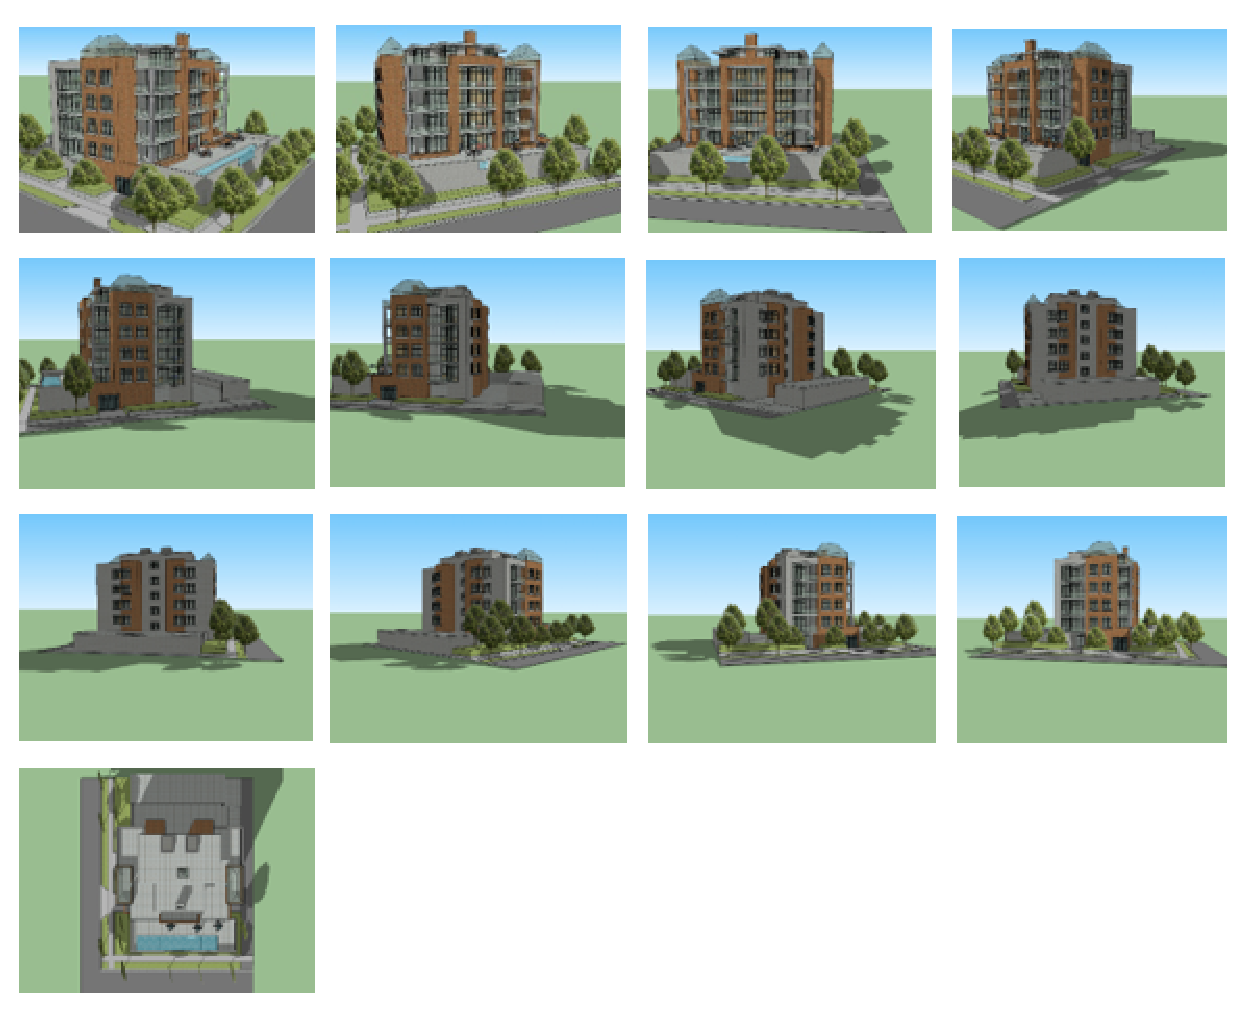
\includegraphics[width=1.0\linewidth]{apartment_building_outdoor}
}
\caption{A 13 sampled scene view images example of an apartment scene model.}
\label{apartment_building_outdoor}
\end{figure}

\end{document}